\section{Literature Review}
\lhead{\leftmark}
\label{sec:review}
\subsection{Numerical Control in Machining}
Numerical Control (NC) is a non-conventional machine control method. A computer program is used to control the machine tool rather than a human operator manually controlling the machining parameters such as the speeds, feeds and depth of cut, as well as the part dimensions. Repeatability and quality are greatly improved over conventional machines. The use of NC machines also reduces non-machining times, such as setup times, tool change times and change of cutting speeds and feeds. It also relieves the operator of tasks such as changing machining parameters(cuttingg speeds and feeds), and locating the tool relative to the work. Even the most simple NC forms, and digital readout equipment, provide much greater accuracy and productivity.
\subsection{CNC Machining}
Computer Numerical Control is an NC method where an on-board microprocessor is directly programmed to control the machine tool. Early NC machines used punched cards for control, while CNC machines use software programming to achieve the machine control.
\subsubsection{The CNC Machining System}
The main components of the CNC system are shown in Fig. \ref{fig:cnc}. These components include:
\begin{enumerate}
	\item The Machine Tool Unit - This is responsible for the extrication work. It consists of the tools to be used, the attachment mechanism, the spindle and all moving parts involved in machining.
	\item The Machine Tool Drives - Classified as either spindle or feed drives. \begin{enumerate}
		\item Spindle drives rotate over a wide range of velocities, measured in rpm.
		\item Feed drives convert angular motion of the motors to linear transverse speeds, measured in mm/min.
	\end{enumerate}
	\item The CNC unit - Runs under a program known as the CNC executive which translates programs written in internationally recognized standard language.
\end{enumerate}
\begin{figure}[h!]
	\centering
	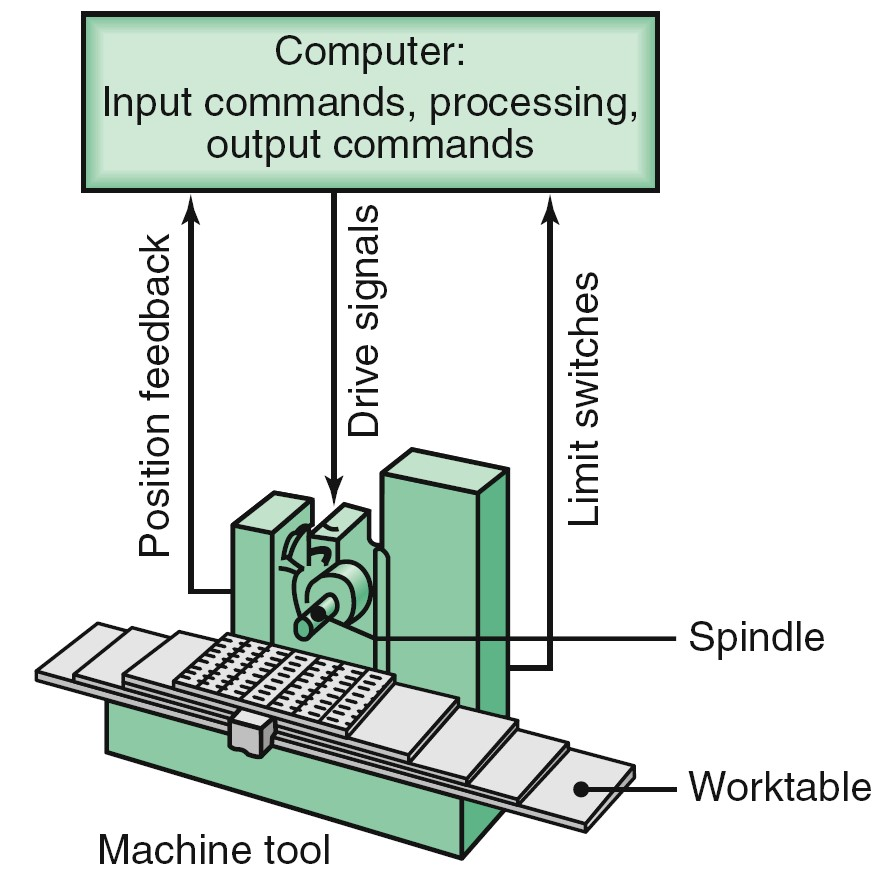
\includegraphics[width=0.8\linewidth]{Figures/cncschematic}
	\caption[CNC Machining System Schematic]{CNC Machine Table Location Schematic \cite{Kalpakjian2010}}
	\label{fig:cnc}
\end{figure}
\subsubsection{CNC Machining Process Parameters}
The CNC Machining Process can be used to machine a number of materials including metals and ceramics. Any material that can be machined conventionally can also be machined using a CNC Milling machine.
The performance of a CNC Machining operation is determined by a number of properties\cite{Kalpakjian2010}:
\begin{enumerate}
	\item Material Removal Rate (MRR)
	\item Surface Quality
	\item Accuracy
	\item Machining time
\end{enumerate}
\subsection{Accuracy in Numerical Control}
Positioning accuracy in numerical-control machines is defined by how accurately the machine can be positioned with respect to a certain coordinate system. \textit{Repeat accuracy} is defined as the closeness of the agreement of the repeated position movements under the same operating conditions of the machine. Resolution, also called sensitivity, is the smallest increment of motion of the machine components.\\
The \textit{stiffness} of the machine tool and the \textit{backlash} in gear drives and leadscrews are important factors in achieving dimensional accuracy. Backlash in modern machines is eliminated by using preloaded ball screws. Also, a rapid response to command signals requires that friction in machine slideways and inertia be minimized. The latter can be achieved by reducing the mass of moving components of the machine—for example, by using lightweight materials, including ceramics.
\newpage
\subsection{Applications}
CNC Machining can be employed in:
\begin{enumerate}
	\item Making complex 3D geometries
	\item Creation of part profiles to be used in making moulds for casting.
	\item Machining centres
	\item Academic/Educational institutions for research and teaching.
\end{enumerate}
\subsection{Other NC Machining Processes}
Numerical control has been applied to a wide variety of other production processes, some of which are listed below\cite{Black2011}:
\begin{enumerate}
	\item NC Punches - Numerical control is used for \textit{X-Y} control on the table.
	\item CNC Lathe machines
	\item CNC Wire EDM Machines
	\item Laser and water-jet abrasive machining
	\item Flame cutters
\end{enumerate}
\subsection{Advantages and Disadvantages of Numerical Control}
Numerical Control has several advantages as compared to other conventional methods of control, some of which are\cite{Kalpakjian2010}:
\begin{enumerate}
	\item Higher production rates, productivity, and product quality; greater operational flexibility; the capacity to make complicated forms with good dimensional precision and repeatability; and reduced scrap loss.
	\item Making machine adjustments is simple.
	\item With each setup, more operations can be completed, and the setup and machining lead times are less than with traditional methods.
	\item Programs can be quickly created and retrieved at any moment.
	\item The level of operator skill needed is lower than that of a skilled machinist, giving the operator more time to focus on other activities around the workspace.
\end{enumerate}
Some of the major limitation of NC machining are:
\begin{enumerate}
	\item Initially expensive cost of the equipment.
	\item The cost of programming and the price of computer time.
	\item The unique maintenance needed.
	\item Preventive maintenance is essential since these equipment are complicated systems and breakdowns can be expensive.
\end{enumerate}